%%%%%%%%%%%%%%%%%%%%%%%%%%%%%%%%%%%%%%%%%
% Beamer Presentation
% LaTeX Template
% Version 1.0 (10/11/12)
%
% This template has been downloaded from:
% http://www.LaTeXTemplates.com
%
% License:
% CC BY-NC-SA 3.0 (http://creativecommons.org/licenses/by-nc-sa/3.0/)
%
%%%%%%%%%%%%%%%%%%%%%%%%%%%%%%%%%%%%%%%%%

%----------------------------------------------------------------------------------------
%	PACKAGES AND THEMES
%----------------------------------------------------------------------------------------

\documentclass{beamer}

\mode<presentation> {

% The Beamer class comes with a number of default slide themes
% which change the colors and layouts of slides. Below this is a list
% of all the themes, uncomment each in turn to see what they look like.

%\usetheme{default}
%\usetheme{AnnArbor}
%\usetheme{Antibes}
%\usetheme{Bergen}
%\usetheme{Berkeley}
%\usetheme{Berlin}
%\usetheme{Boadilla}
%\usetheme{CambridgeUS}
%\usetheme{Copenhagen}
%\usetheme{Darmstadt}
%\usetheme{Dresden}
%\usetheme{Frankfurt}
%\usetheme{Goettingen}
%\usetheme{Hannover}
%\usetheme{Ilmenau}
%\usetheme{JuanLesPins}
%\usetheme{Luebeck}
\usetheme{Madrid}
%\usetheme{Malmoe}
%\usetheme{Marburg}
%\usetheme{Montpellier}
%\usetheme{PaloAlto}
%\usetheme{Pittsburgh}
%\usetheme{Rochester}
%\usetheme{Singapore}
%\usetheme{Szeged}
%\usetheme{Warsaw}

% As well as themes, the Beamer class has a number of color themes
% for any slide theme. Uncomment each of these in turn to see how it
% changes the colors of your current slide theme.

%\usecolortheme{albatross}
%\usecolortheme{beaver}
%\usecolortheme{beetle}
%\usecolortheme{crane}
%\usecolortheme{dolphin}
%\usecolortheme{dove}
%\usecolortheme{fly}
%\usecolortheme{lily}
%\usecolortheme{orchid}
%\usecolortheme{rose}
%\usecolortheme{seagull}
%\usecolortheme{seahorse}
%\usecolortheme{whale}
%\usecolortheme{wolverine}

%\setbeamertemplate{footline} % To remove the footer line in all slides uncomment this line
%\setbeamertemplate{footline}[page number] % To replace the footer line in all slides with a simple slide count uncomment this line

%\setbeamertemplate{navigation symbols}{} % To remove the navigation symbols from the bottom of all slides uncomment this line
}

\usepackage{graphicx} % Allows including images
\usepackage{booktabs} % Allows the use of \toprule, \midrule and \bottomrule in tables
\usepackage{listings}
\usepackage{amsmath}
\usepackage{algpseudocode,algorithm,algorithmicx}

\lstdefinestyle{customjava}{
  breaklines=true,
  frame=L,
  xleftmargin=\parindent,
  language=Java,
  showstringspaces=false,
  basicstyle=\footnotesize\ttfamily,
  keywordstyle=\bfseries\color{green!40!black},
  commentstyle=\itshape\color{gray!40!black},
  identifierstyle=\color{blue},
  stringstyle=\color{orange},
}

\lstdefinestyle{customcpp}{
  breaklines=true,
  frame=L,
  xleftmargin=\parindent,
  language=C++,
  showstringspaces=false,
  basicstyle=\footnotesize\ttfamily,
  keywordstyle=\bfseries\color{green!40!black},
  commentstyle=\itshape\color{gray!40!black},
  identifierstyle=\color{blue},
  stringstyle=\color{orange},
}
%----------------------------------------------------------------------------------------
%	TITLE PAGE
%----------------------------------------------------------------------------------------

\title[Processes 1]{Processes 1} % The short title appears at the bottom of every slide, the full title is only on the title page

\author{Jonathan Windle} % Your name
\institute[UEA] % Your institution as it will appear on the bottom of every slide, may be shorthand to save space
{
University of East Anglia \\ % Your institution for the title page
\medskip
\textit{J.Windle@uea.ac.uk} % Your email address
}
\date{\today} % Date, can be changed to a custom date

\begin{document}

\begin{frame}
\titlepage % Print the title page as the first slide
\end{frame}

\begin{frame}[allowframebreaks]
\frametitle{Overview} % Table of contents slide, comment this block out to remove it
\tableofcontents % Throughout your presentation, if you choose to use \section{} and \subsection{} commands, these will automatically be printed on this slide as an overview of your presentation
\end{frame}

%-------------------------------------------------------------------
\section{POSIX}
\begin{frame}
\frametitle{POSIX}
\begin{itemize}
\item For programs to run on any UNIX system IEEE developed a standard for UNIX called POSIX.
\item Defines a minimal system cll interface comprising of about 100 procedure calls.
\item Grouped into four categories:
\begin{itemize}
\item Process management
\item File management
\item Directory and file system management
\item Miscellaneous.
\end{itemize}
\end{itemize}
\end{frame}
%--------------------------------------------------------------------
\section{Multiprogramming}
\begin{frame}
\frametitle{Multiprogramming}
\begin{itemize}
\item CPU switches from program to program running each for 10s of milliseconds.
\item Creates an illusion of parallelism sometimes called pseudo-parallelism
\item System designers have developed a conceptual model called sequential processes to keep track of multiple parallel activities.
\item Most programs are sequential processes.
\item They comprise of a series of instructions, executed sequentially.
\item Assuming the input is unchanged they will always produce the same result.
\end{itemize}
\end{frame}
%-------------------------------------------------------------------
\subsection{Three Views}
\begin{frame}
\frametitle{Three views of Multi-programmings}
\begin{itemize}
\item Computer multiprogramming four programs in memory.
\item Four processes each with its own flow of control.
\item Trace of ecevution shows all processes making progress.
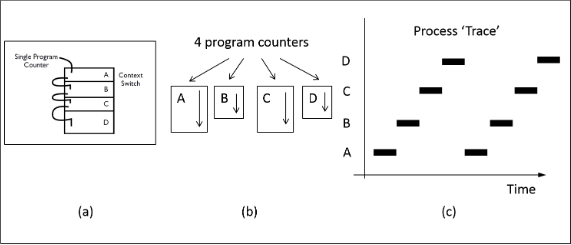
\includegraphics[scale=0.5]{three.png}
\end{itemize}
\end{frame}
%--------------------------------------------------------------
\subsection{Side Effects}
\begin{frame}
\frametitle{Side Effects}
\begin{itemize}
\item Because of CPU switching, the rate at which a process performs its computation will not be uniform and probably not even be reproducible if the same processes are run again.
\item Processes must \textbf{NOT} be programmed with built in assumptions about timing.
\item When a process has a particular critical real-time requirement meaning particular events must occur within a specified number of milliseconds, special measures must be taken.
\end{itemize}
\end{frame}
%------------------------------------------------------------------
\subsection{Process vs Program}
\begin{frame}
\frametitle{Process vs Program}
\begin{itemize}
\item Key idea is that a process is an activity of some kind.
\item It has a:
\begin{itemize}
\item Program
\item Input
\item State
\item Output
\end{itemize}
\item A single processor may be shared amongst several processes.
\item A process is a program in execution.
\item A program is just a list of instructions in memory.
\end{itemize}
\end{frame}
%-------------------------------------------------------------------
\subsection{Process Creation}
\begin{itemize}
\item OS need some way to create and terminate processes.
\item Four principle events cause processes to be created:
\begin{itemize}
\item System initialisation
\item Execution of a process creation system call (by another process)
\item A user types a command.
\item A user runs a batch job.
\end{itemize}
\item In UNIX there is only one system call for creating a process: \texttt{fork}.
\item \texttt{fork} creates an exact clone of the calling process. After \texttt{fork} there are two processes, the parent and the child, each having:
\begin{itemize}
\item Their own {\color{red}distinct address space}.
\item The same {\color{green}memory image}.
\item The same {\color{purple}environment settings}
\item The same {\color{orange}open files}
\end{itemize}
\item Usually the child process then executes \texttt{execve} to change its memory image and run a new program.
\end{itemize}
%------------------------------------------------------------------
\subsection{Process Termination}
\begin{frame}
\frametitle{Process Termination}
\begin{itemize}
\item Terminate due to:
\begin{itemize}
\item Normal exit (voluntary).
\item Error exit (voluntary)
\item Fatal error (involuntary)
\item Killed by another process (involuntary). 
\end{itemize}
\end{itemize}
\end{frame}
%-------------------------------------------------------------------
\subsection{Process Hierarchies}
\begin{frame}
\frametitle{Process Hierarchies}
\begin{itemize}
\item Some systems, when a process creates another process, the parent process and child process cnotinue to be associated.
\item In UNIX, a process and all its children form a process group e.g.:
\begin{itemize}
\item When a user sends a signal from the keyboard it is sent to all members of the prcess group currently associated with the keyboard.
\item When UNIX is started, \texttt{init} is present in the boot image. When it starts running, it reads a file telling how many terminals there are and \texttt{forks} one new process per terminial. It waits for a user to log in and if login is successful the login process executes a shell to accept commands. Hence, in UNIX all the proceses in the whole system belong to a single tree, with \texttt{init} at the rot.
\end{itemize}
\item \texttt{pstree} command shows the running processses as a tree.
\end{itemize}
\end{frame}
%------------------------------------------------------------------
\subsection{Process States}
\begin{frame}
\frametitle{Process States}
\begin{columns}[c]
\column{.5\textwidth}
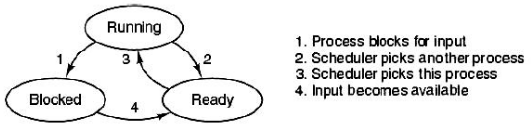
\includegraphics[scale=0.35]{state1.png}
\column{.5\textwidth}
\begin{itemize}
\item Transition 1 occurs when the S discovers that the process cannot continue right now.
\item Transition 2 \& 3 are caused by the schedular (part of OS).
\item Transition 4 occurs when the external event for which the process was waiting (such as arrival of input) happens.
\item External events send electrical signals called interrupts to the schedular.
\end{itemize}
\end{columns}
\end{frame}
%-----------------------------------------------------------------
\subsection{Process Model}
\begin{frame}
\frametitle{Process Model}
\begin{columns}[c]
\column{.5\textwidth}
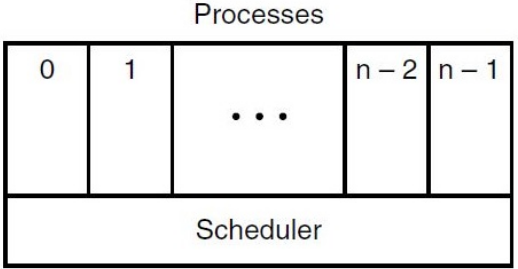
\includegraphics[scale=0.35]{sched.png}
\column{.5\textwidth}
\begin{itemize}
\item Using process model, becomes much easier t think about what's going on inside the system.
\item In the process model, the lowest level of the OS is the {\color{red}schedular} with a variety of proesses on top of it.
\item All of the details of interrupt handling and actually starting and stopping te processes is hidden away in the {\color{red}schedular}.
\end{itemize}
\end{columns}
\end{frame}
%------------------------------------------------------------------
\subsection{Implementation of Processes}
\begin{frame}
\frametitle{Implementation of Processes}
\begin{columns}[c]
\column{.5\textwidth}
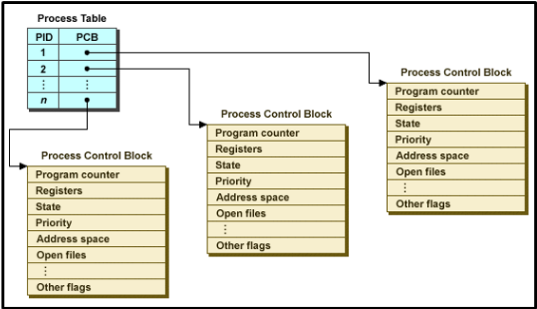
\includegraphics[scale=0.35]{ptable.png}
\column{.5\textwidth}
\begin{itemize}
\item The OS maintains a table called the {\color{red}process table}.
\item Individual entries in the tabel calles {\color{green}process control blocks} hold important information about the process state:
\begin{itemize}
\item Program counter
\item Stack pointer
\item Memory allocation
\item Open files
\item Other accounting and scheduling information
\end{itemize}
\end{itemize}
\end{columns}
\end{frame}
%-------------------------------------------------------------------
\subsection{Modelling Multiprogramming}
\begin{frame}
\frametitle{Modelling Multiprogramming}
\begin{columns}[c]
\column{.5\textwidth}
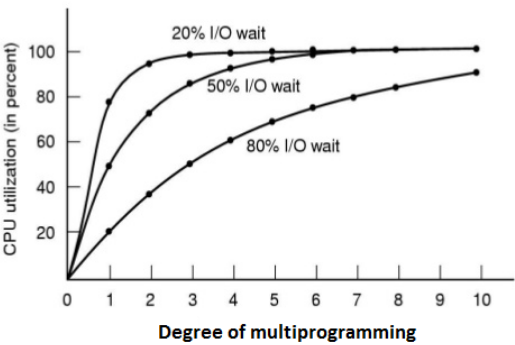
\includegraphics[scale=0.35]{util.png}
\column{.5\textwidth}
\begin{itemize}
\item Model CPU usage from a probabilistic viewpoint.
\item Suppose that a process spends a fraction of its time $p$ waiting for I/O to complete.
\item Assum $n$ processes in memory at once.
\item Probability that all $n$ process will be waiting for I/O is $p^n$,
\item Hence, CPU Utilisation = $1-p^n$
\end{itemize}
\end{columns}
\end{frame}
%------------------------------------------------------------------
\subsection{Execution Modes}
\begin{frame}
\frametitle{Execution Modes}
\begin{columns}[c]
\column{.5\textwidth}
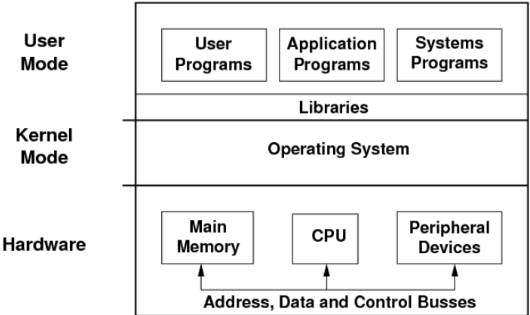
\includegraphics[scale=0.35]{exec.png}
\column{.5\textwidth}
\begin{itemize}
\item Most computers have two mode of execution:
\begin{itemize}
\item Kernel (or supervisor) Mode.
\item User Mode
\end{itemize}
\item Processes running in kernel mode have unrestricted access to the machine:
\begin{itemize}
\item The can disable all interrupts
\item Manipulate stacks
\item Unrestricted access to memory and I/O.
\end{itemize}
\end{itemize}
\end{columns}
\end{frame}
%--------------------------------------------------------------------
\section{Threads}
\begin{frame}
\frametitle{Threads}
\begin{itemize}
\item In traditional OS, each process has an address space and a single thread of execution.
\item It is sometimes desirable to have multiple threads of control in the same address space running in quasi-parrallel.
\item Threads run as though they were (almost) seperate processes (excpet for the shared address space).
\item A thread can be considered a {\color{red}lightweight} process.
\end{itemize}
\end{frame}
%-----------------------------------------------------------------
\subsection{Single-Threaded vs Multithreaded Processes}
\begin{frame}
\frametitle{Single-Threaded vs Multithreaded Processes}
Multithreaded partition of kernel / User space assumes threads are implemented in user space.
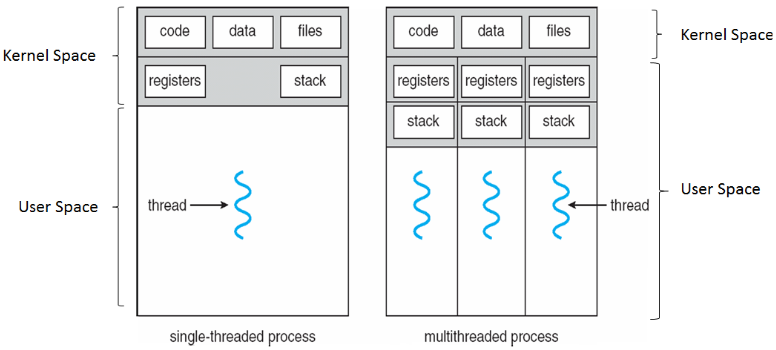
\includegraphics[scale=0.45]{thread.png}
\end{frame}
%--------------------------------------------------------------------
\subsection{Advantages of Threads}
\begin{frame}
\frametitle{Advantages of Threads}
\begin{itemize}
\item Decomposing the application into multiple threads that run in quasi-parallel the progrmming model becomes simpler. Also, threads share the same address space and data (unlike processes).
\item Since threads are lighter weight than processes they are easier to create and destroy than processes. Creating a thread is typically 10-100 times quicker than creating a process.
\item Threads are useful on systems with multiple CPUs.
\item Threads yield no performance gain when all of them are CPU bound.
\item Multiple threads are appropriate when they are part of the same job and actively cooperating with one another.
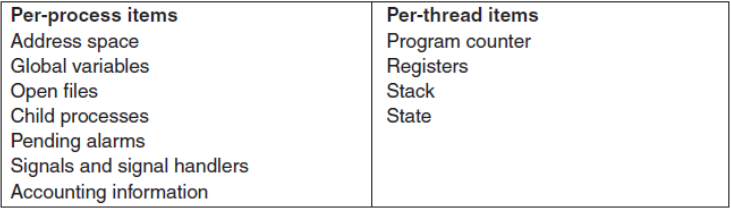
\includegraphics[scale=0.2]{adv.png}
\end{itemize}
\end{frame}
%-----------------------------------------------------------------
\subsection{Thread States}
\begin{frame}
\frametitle{Thread States}
\begin{columns}[c]
\column{.5\textwidth}
\column{.5\textwidth}
\begin{itemize}
\item A thread can be in one of three states:
\begin{itemize}
\item Running
\item Blocked
\item Ready
\end{itemize}
\item Different ways it can be blocked:
\begin{itemize}
\item When the process blocks, ALL threads block
\item Threads may block waiting for an event
\item Threads may enter a sleep state to be woken by a signaal from another thread.
\end{itemize}
\end{itemize}
\end{columns}
\end{frame}
%------------------------------------------------------------------
\subsection{Implementing Threads}
\begin{frame}
\frametitle{Implementing Threads}
Threads can be implemented in user space or kernel space
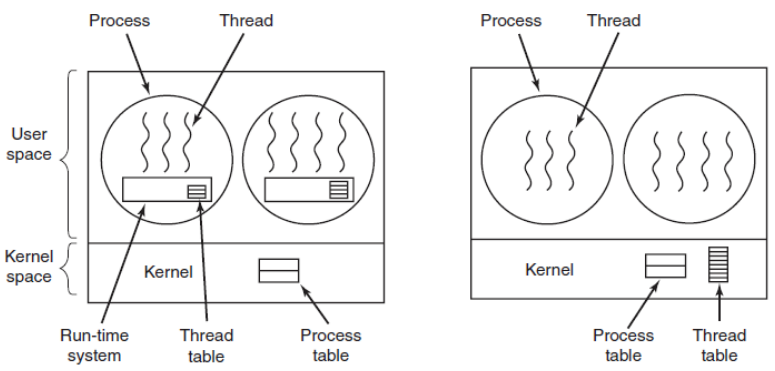
\includegraphics[scale=0.4]{thr.png}
\end{frame}
%----------------------------------------------------------------
\subsection{Threads in User Space}
\begin{frame}
\frametitle{Threads in User Space}
\begin{itemize}
\item Advantages:
\begin{itemize}
\item As far as the kernel is concerned it is running one single threaded process.
\item Can be run on OS that doesn't support multithreading.
\item Thread switching can be made very fast.
\item Each process can have its own scheduling algorithm for threads.
\end{itemize}
\item Disadvantages:
\begin{itemize}
\item If a thread starts running, no other thread in that process will ever run unless the first thread gives up the CPU.
\item Blocking system calls are difficult to implement.
\item Progrmammers generally want threads precisely in applications where the threads block often, and its more efficient to implement as a process.
\end{itemize}
\end{itemize}
\end{frame}
%-----------------------------------------------------------------
\subsection{Threads in Kernel Space}
\begin{frame}
\frametitle{Threads in Kernel Space}
\begin{itemize}
\item Advantages:
\begin{itemize}
\item Kernel threads do not require any new, nonblocking system calls.
\end{itemize}
\item Disadvantages:
\begin{itemize}
\item The cost of creating and destroying threads in the kernel is substatial.
\item All calls that might block a thread are implemented as system calls at considerable greater cost than a call to a run-tme system procedure.
\end{itemize}
\item Other issues:
\begin{itemize}
\item What happens when the process \texttt{forks}?
\item How can we handle signals?
\end{itemize}
\end{itemize}
\end{frame}
%-------------------------------------------------------------------
\section{Summary}
\begin{frame}
\frametitle{Summary}
\begin{itemize}
\item Processes are Ready,Running or Blocked.
\item Threads may also Sleep and Wait.
\item Two modes of execution User \& Kernel processes switch to kernel mode during system calls.
\item Threads are lightweight processes.
\item Two types of thread implementations:
\begin{itemize}
\item Kernel threads: Managed by the OS
\item User threads: Managed by user.
\end{itemize}
\end{itemize}
\end{frame}
%------------------------------------------------------------------

\begin{frame} 
\Huge{\centerline{The End}}
\end{frame}

\end{document}